\section{Introduction}

The lack of consensus on Password Composition Policies (PCPs) and the lack of adoption of best practices on the web~\cite{lee_password_2022} suggest that our knowledge of password security is not yet complete. Password Strength Meters (PSMs), such as the \zxcvbn PSM, which was found to be the best dictionary-based PSM by Wang~\etal~\cite{wang_no_2023} and has 14.7K GitHub stars, still have obvious weak points. For example, \zxcvbn gives the password \password{girlsruledaworld} a maximum score of 4 (scores range from 1 to 4). It also assigns a strong score of 3/4 to \password{asdf1fdsa1}. This is because PSMs such as \zxcvbn depend on the patterns and structures they are programmed to recognise. This raises the question of what other patterns we are missing. To advance our understanding of passwords, we provide the first human-labelled password dataset.

\begin{figure}[t]
    \centering
    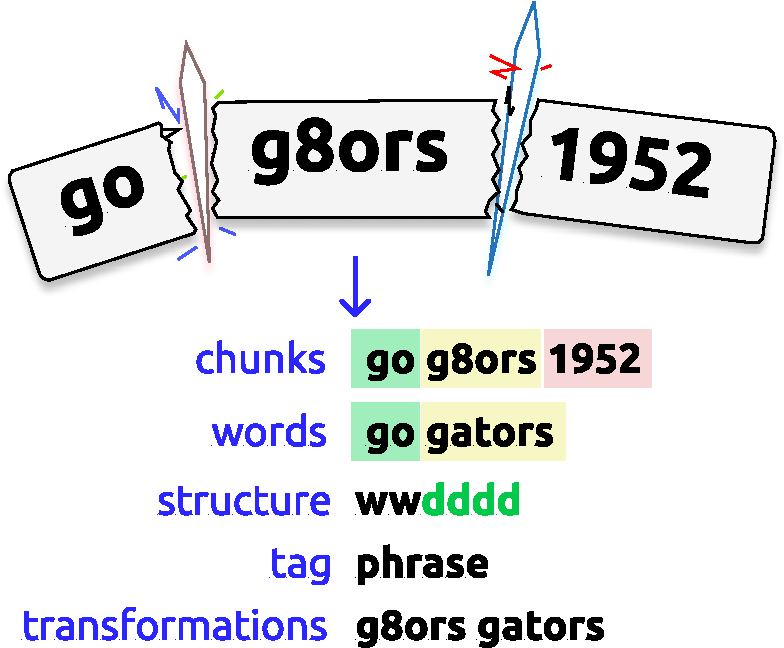
\includegraphics[scale=0.5]{figs/why_passwords/intro_fig.pdf}
    \caption{Example of the labelling process. The password \texttt{gog8ors1952} is sliced into core constituents, then the meaningful words are extracted. Such a labelling process can capture details such as transformations. \srcOwnFig}
    \label{fig:intro_password}
    %\vspace{-1em} % Adjust the negative value to reduce the gap
\end{figure}

It is almost common knowledge that we embed personal information in our secrets and that they possess a certain structure. But have we studied and collected most of these patterns and structures? The implications are important, as we saw with the \zxcvbn example---users can be misled into believing their secrets are strong enough. Other fields benefit from a plethora of labelled datasets that can be analysed; unfortunately, such a dataset does not exist in web security, specifically in password security. The chief task of this chapter is to human-label such a dataset and propose new methods to advance our understanding of password compositions.

We manually label the \hmail (2009) dataset~\cite{miessler_hotmail_2009} and machine-label the Lizard Squad dataset (2015)~\cite{miessler_lizardsquad_2015}. We are also in the process of fully labelling the Fortinet (2022) dataset~\cite{miessler_fortinet_2021}. The dataset itself is the key contribution of this chapter, and we discuss many implications in Section~\ref{sec::passwordninja::discussion}. In Section~\ref{sec::chp4::results}, we provide the results of an analysis on the \hmail dataset and consequently list a more comprehensive set of transformations and structures that can be applied to PSMs such as \zxcvbn.

We address the ethical issue of working with compromised data. We have constrained ourselves to the SecLists datasets~\cite{miessler_danielmiesslerseclists_2024} to ensure that we do not release any new material. Additionally, we have taken measures to prevent the release of any personally identifiable information (PII). Moreover, these datasets have been extensively used in numerous password-guessing algorithms and prior literature, and the practice of using real password datasets is well established. We discuss this further in Section~\ref{passwordninja::ethicalconsiderations}.


Understanding password composition is critical in password modelling, as it significantly impacts the precision and efficacy of predictive models. Traditional methods, such as~\cite{narayanan_fast_2005}, typically analyse passwords at the character level, considering the likelihood of each character's occurrence in sequence. More sophisticated techniques, like chunking~\cite{Xu_Wang_Yu_Zhang_Zhang_Han_2021}, break down passwords into larger, meaningful segments rather than isolated characters, offering a refined perspective on password composition. Nonetheless, these approaches do not provide the detailed insight needed to fully understand nuances such as word transformations, semantic contexts, and structural patterns within passwords.

Data labelling is highly time-consuming and expensive. Thus, we asked ourselves: how can we expedite the labelling process? We can either hire more human agents or develop algorithms and models for assistance. We tested both approaches, employing paid freelancers and utilising language models to aid in the labelling process (see Section~\ref{section:experiment1}).


\textbf{Contributions of this chapter:}

\begin{enumerate}
\item \textbf{Human-Labelled Password Corpus.} (Section~\ref{sec::chp4::results}) We decompose and label the \hmail~2009~\cite{miessler_hotmail_2009} password strings (\num{8292}) into chunks, words, structure, tags, and transformations, where applicable. Using the methods developed in Section~\ref{section:experiment1}, we machine-label the \lizardsquad~2015 dataset~\cite{miessler_lizardsquad_2015}. To our knowledge, this is the first dataset of its kind. Insights derived from our labelled dataset are discussed, and the dataset is made available for research\footnote{\passwordNinjaURL}.

\item \textbf{Password Composition.} (Section~\ref{sec::chp4::pcp}) Utilising our labelled dataset, we evaluate secure and practical password composition strategies. We find that password structures, such as three-word passphrases without semantic links between words, offer both security and practicality. The use of the \hmail~2009 dataset and the Lizard Squad~2015 dataset provides an opportunity to investigate changes in password composition over time and to reflect on the relevance of these datasets given their age. Using a novel mathematical framework and empirical analysis we recommend a five-word PCP.

\item \textbf{Large Language Models and Human Labellers.} (Section~\ref{section:experiment1}) Labelling data is time-consuming and costly, prompting exploration of alternatives to expedite the process. We engaged freelancers from Fiverr~\cite{fiverr2024} and assessed their work against Large Language Models in terms of accuracy, cost, and time. The preliminary results indicate that language models are a promising tool for further experimentation.
\end{enumerate}